\section{Evaluation}
\label{evaluation}
Figure \ref{fig:program} is an social network program wrote in Jeeves, which describes how to introduce sensitive values, use them to compute result values, and display the results in defferent output contexts. And Figure \ref{fig:result} is the corresponding result after executing this program in Haskell 98\footnote{https://www.haskell.org/hugs/} environment.
\begin{figure}[h]
    \centering
    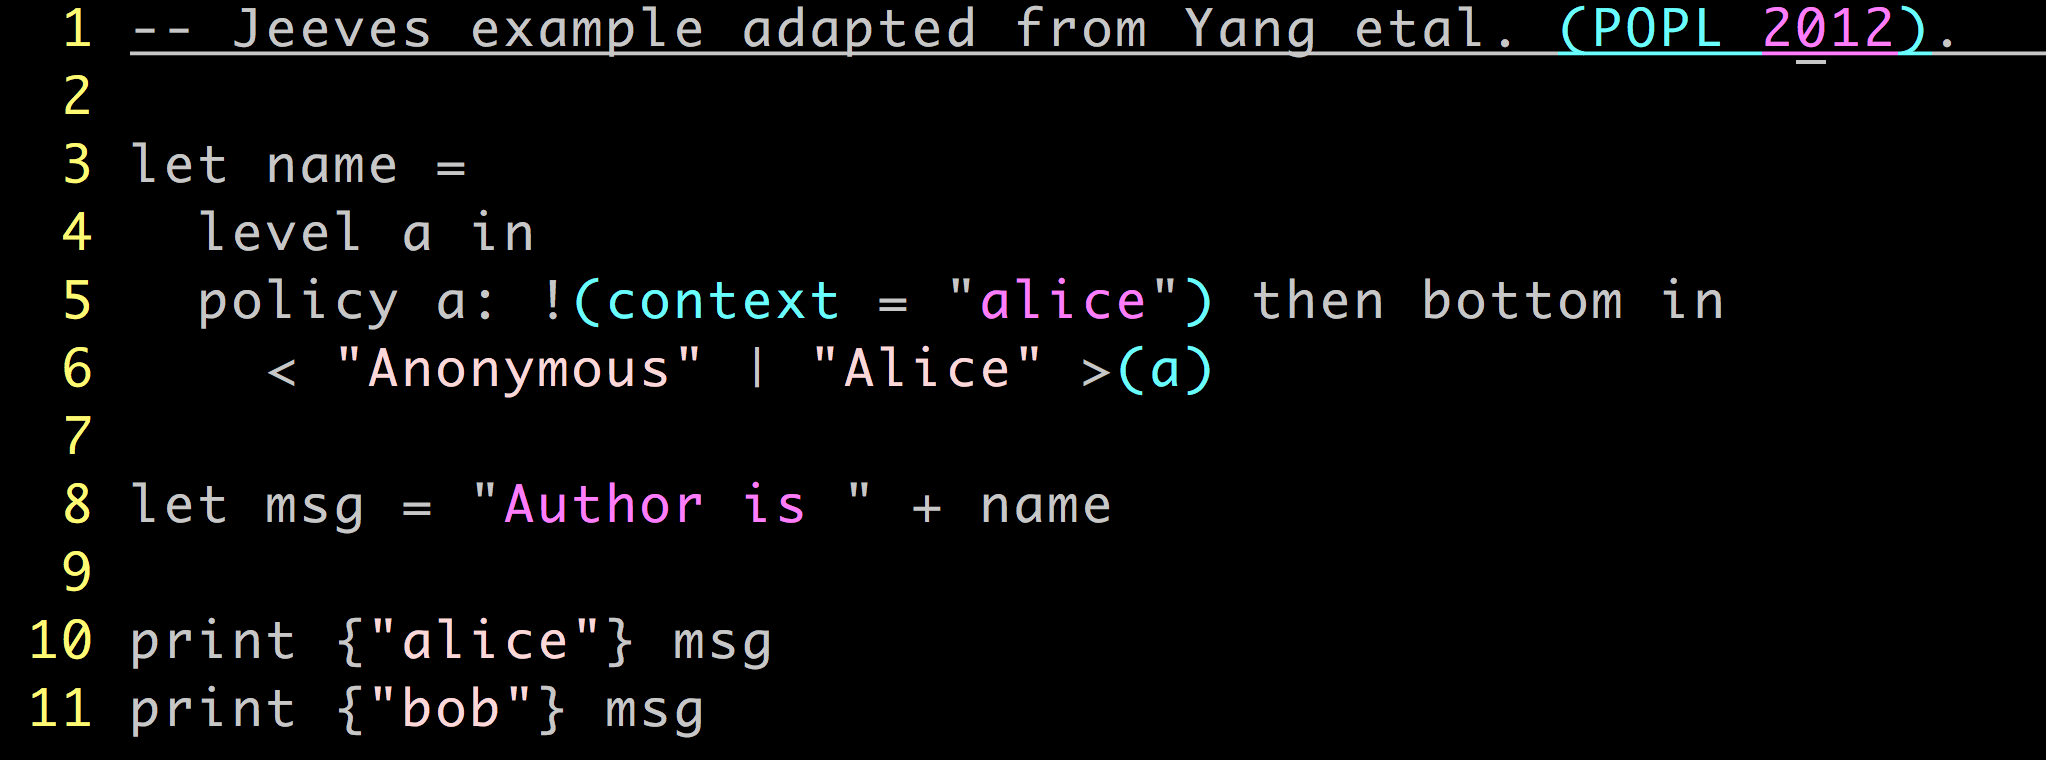
\includegraphics[width=1.0\textwidth]{program.PNG}
    %\vspace*{-.6cm}
    \caption{Source program example}
    \label{fig:program}
\end{figure}

The following haskell source code describe the syntax of the $\lambdaJ$ language.
\begin{lstlisting}[language=Haskell]
    data Exp = E_BOOL Bool | E_NAT Int 
                    | E_STR String | E_CONST String  
                    | E_VAR Var   | E_CONTEXT 
                    | E_LAMBDA Var Exp | E_THUNK Exp 
                    | E_OP Op Exp Exp  | E_UOP UOp Exp                    
                    | E_IF Exp Exp Exp | E_APP Exp Exp                   
                    | E_DEFER Var Exp | E_ASSERT Exp Exp                  
                    | E_LET Var Exp Exp                   
                    | E_RECORD [(FieldName,Exp)] 
                    | E_FIELD Exp FieldName
                    deriving (Ord,Eq)
    
    data Op = OP_PLUS | OP_MINUS
                    | OP_LESS | OP_GREATER 
                    | OP_EQ | OP_AND | OP_OR | OP_IMPLY
                    deriving (Ord,Eq)
    
    data UOp = OP_NOT   deriving (Ord,Eq) 
    
    data FieldName = FIELD_NAME String  deriving(Ord,Eq)
    data Var = VAR String deriving (Ord,Eq)
\end{lstlisting}

%\begin{verbatim}
% ---------
% let name =  
%     level a in
%     policy a: !(context = alice) then bottom in < "Anonymous" | "Alice" >(a)
% 
% let msg = "Author is " + name
% 
% print {alice} msg
% print {bob} msg
% ------
%\end{verbatim}

\begin{figure}[h]
    \centering
    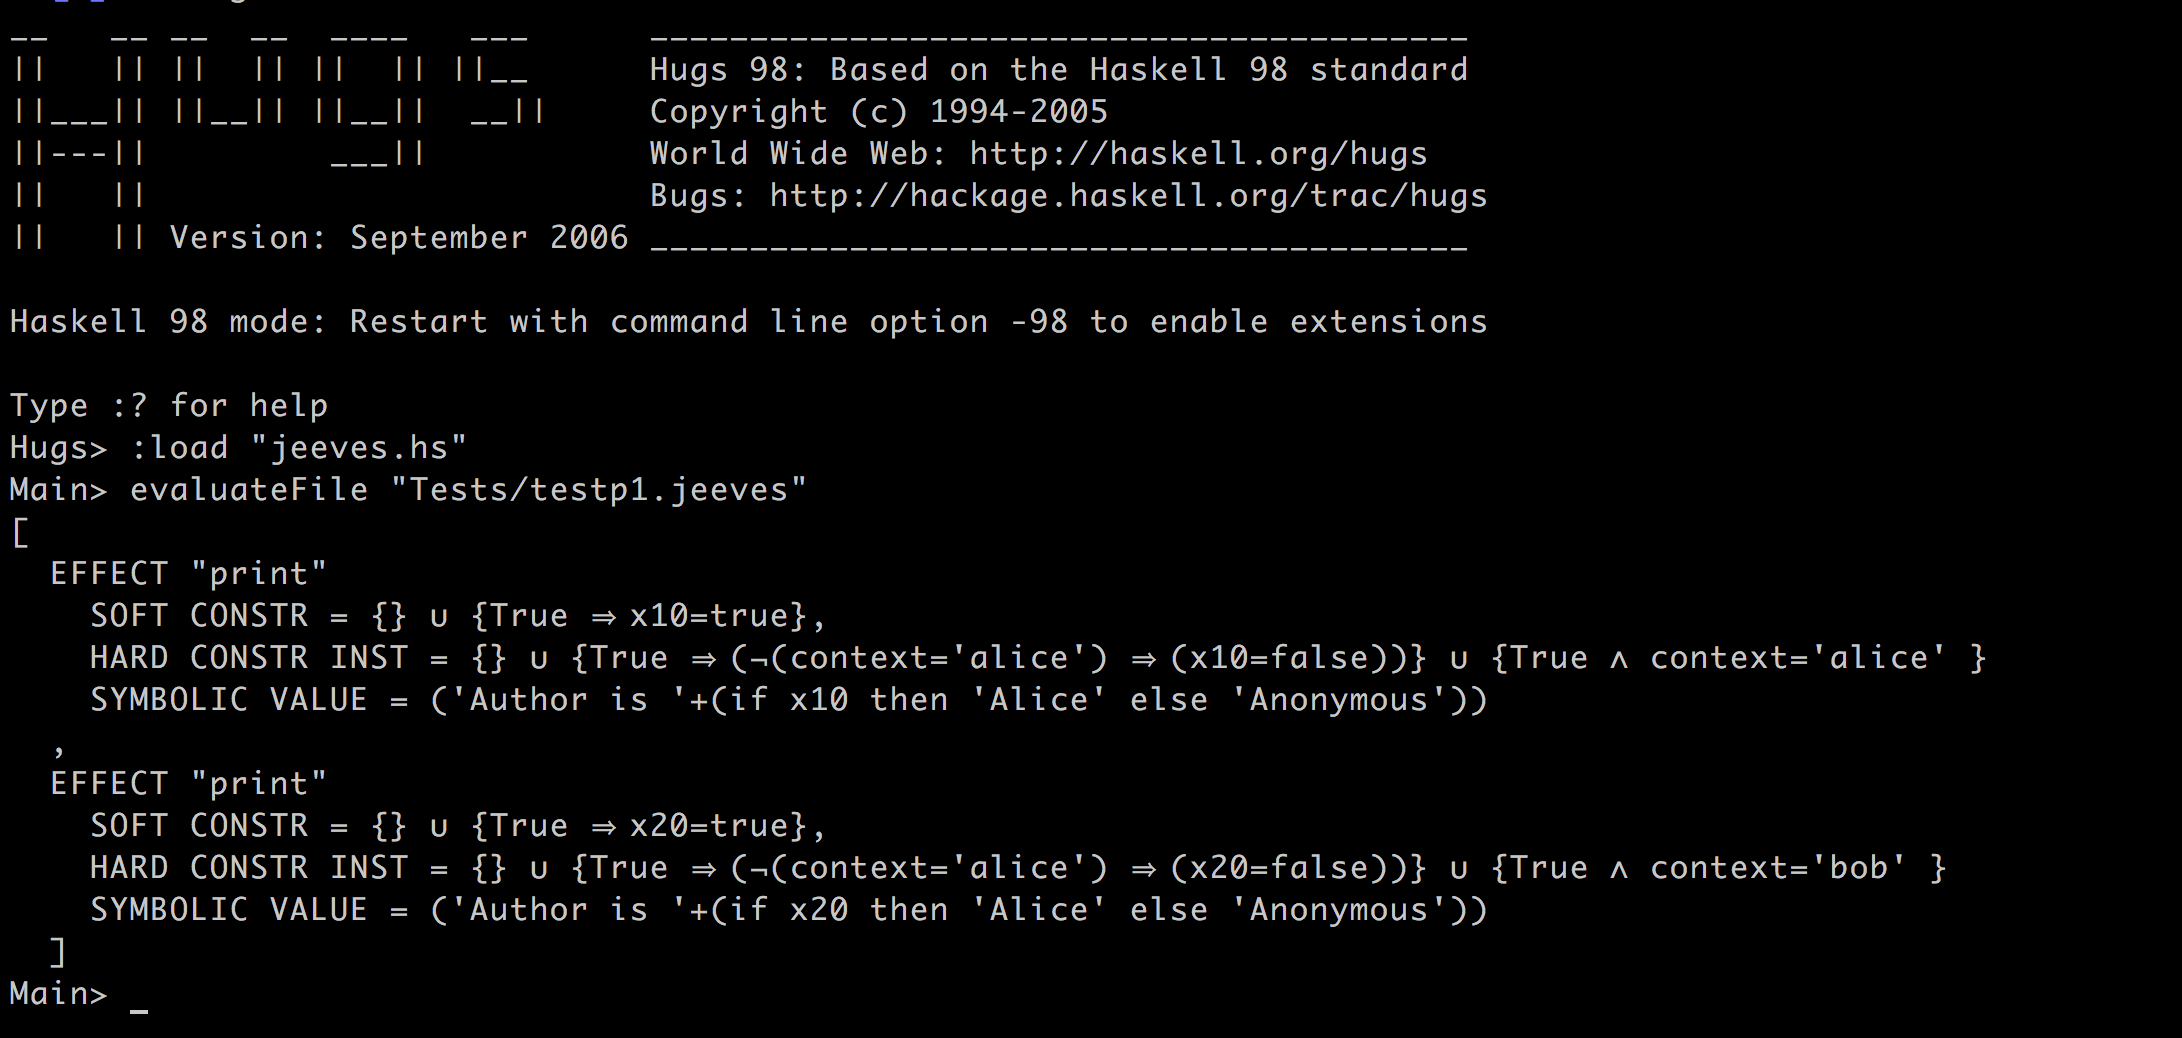
\includegraphics[width=1.0\textwidth]{result.PNG}
    %\vspace*{-.6cm}
    \caption{Execution result}
    \label{fig:result}
\end{figure}


